\documentclass[tikz,border=3.14mm]{standalone}
\usepackage{tikz}
\usepackage{physics}
\usepackage{xcolor}
\usetikzlibrary{shadings, angles, quotes}

\begin{document}
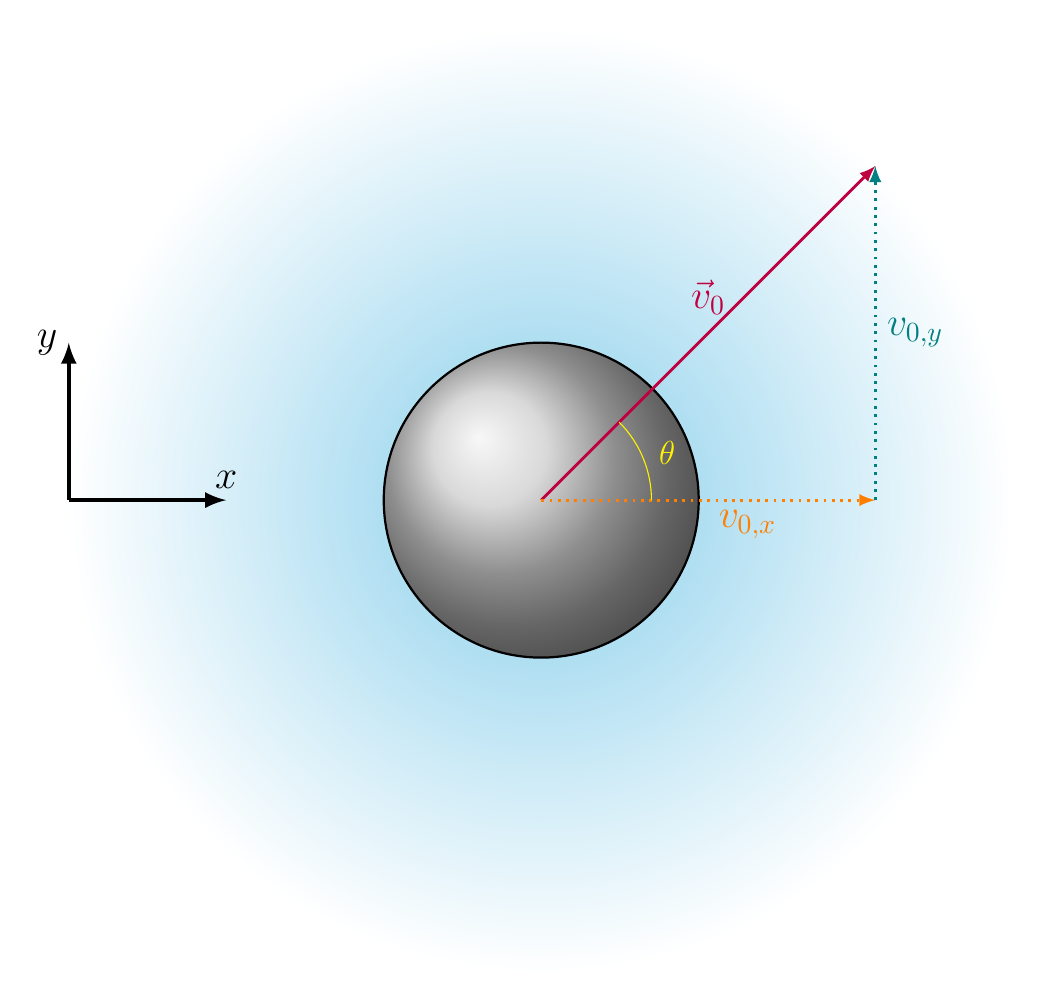
\begin{tikzpicture}[scale=2]

% Define velocity
\def\velocityLength{3}

% Define skyblue color
\definecolor{skyblue}{RGB}{135,206,235}

% Draw background as a sky
\shade[inner color=skyblue, outer color=white] (-3,-3) rectangle (3,3);

% Draw bullet as a shaded circle for a 3D effect
\shade[ball color=gray!40] (0,0) circle (1cm);

% Draw bullet outline to make it more visible
\draw[thick] (0,0) circle (1cm);

% Draw velocity at theta degree angle from the center of the bullet
\draw[-latex, line width=1pt, purple] (0,0) -- ++(45:\velocityLength) node[midway,above, yshift=0.1cm] {\Large $\vec{v}_0$}; % Initial Velocity

% Draw velocity components
\draw[dotted, -latex, line width=1pt, orange] (0,0) -- ++(0:\velocityLength*cos 45) node[midway,below, xshift=0.5cm] {\Large $v_{0,x}$}; % x-component
\draw[dotted, -latex, line width=1pt, teal] (\velocityLength*cos 45,0) -- ++(90:\velocityLength*sin 45) node[midway,left, xshift=1cm] {\Large $v_{0,y}$}; % y-component

% Draw angle theta
\draw[thin, yellow] (0.7cm,0) arc (0:45:0.7cm);
\node at (0.8cm,0.3cm) {\large \textcolor{yellow}{$\theta$}};

% Draw coordinate axes
\draw[-latex, ultra thick] (-3,0) -- (-2,0) node[above] {\Large $x$};
\draw[-latex, ultra thick] (-3,0) -- (-3,1) node[left] {\Large $y$};

\end{tikzpicture}
\end{document}
